\documentclass[a4paper,12pt]{article}
\usepackage[ngerman]{babel}
\usepackage[utf8]{inputenc}

\usepackage{amsbsy,amsmath,amsthm,amssymb}
\usepackage{amsfonts,enumerate}
\usepackage{verbatim,color}
\usepackage{graphicx}
\usepackage{enumitem}
\usepackage[breaklinks=true]{hyperref}

%\setlength{\oddsidemargin}{-1.cm}
%\setlength{\evensidemargin}{-1.cm}
%\setlength{\textheight}{23.5cm}
%\setlength{\textwidth}{16cm}

\setlength{\topmargin}{-1cm}
\setlength{\textheight}{22.5cm}
\setlength{\textwidth}{16cm}
\setlength{\oddsidemargin}{0cm}
\setlength{\evensidemargin}{0cm}
\setlength{\parindent}{0pt}

\newcommand{\RR}{{\mathbb R}}
\newcommand{\code}{\texttt}

\headsep = 0pt
\textheight = 700pt

\begin{document}
\begin{titlepage}
\centering
\vspace*{5cm}

 \includegraphics[width = 1\textwidth]{LEDtrix_Logo.png}
\vspace{1cm}

\large{Computer Architecture and Operating Systems\\Fall semester 2018}
\end{titlepage}
 
 \section{Introduction}
 
 LEDtrix is a square LED matrix encased by a box made of wood. A connected RaspberryPi with two buttons are controlling the system, allowing users to play some games on the board.
 Our aim is to assemble all parts, to have at least two running games and an easy expandable code, so adding a new game can be done quickly.
 We think that updating the pixels continuously whilst calculating the game logic, could be a challenging task to master.
 Not accomplishing the last point would result in flickering LEDs and therefore drastically worsen the gaming experience.
 Due to this importance it must be well thought out so that a desired result can be achieved.
 
 \section{Background}
 
 The idea for our project came by coffee tables containing LED matrices.
 We liked this idea and thought of a way to produce something similar, being easier to transport.
 Since the product must be able to withstand displacements, the decision to produce a wooden frame for protection was made quickly.
 Then, we had to think about how to control the games.
 After a quick evaluation of touch pads, we suddenly came up with the concept of adding two buttons (reference 3).
 With this approach, we could keep the game logic as simple as possible, concentrating on the more important and interesting parts of the project.
 
 Seeing that we both had no experience with soldering, especially as it would have taken all of the available project time, we decided on using LED strips instead of 225 separate ones.
 After looking up the major differences between some models, we found out that we need the APA102 (references 1 and 2).
 They have a clock line and are therefore better for us, compared to the WS2812 LEDs which do not have one.
 With the other LEDs we would have run into serious problems.
 Transferring data to the LEDs in very small and exactly defined time slots is not possible with software running on top of a non real-time operating system.

\section{Building the box}
 We began by building the box, continued by fixating the LED strips and soldering them together.
 Our first problems arose when we tried to splice the wooden slats.
 For that we went to the switchgear workshop of Elektrizitäts AG Basel (reference 5), where we realised that this would be very unstable.
 The employees helped us build a stronger box by screwing the pieces together instead of using glue.
 The pictures below show one of the employees helping us to saw the wood (left) and one of us drilling a screw hole into a metal plate which will then strengthen one of the four box corners (right).
 
\vspace{1cm}

{ \centering
  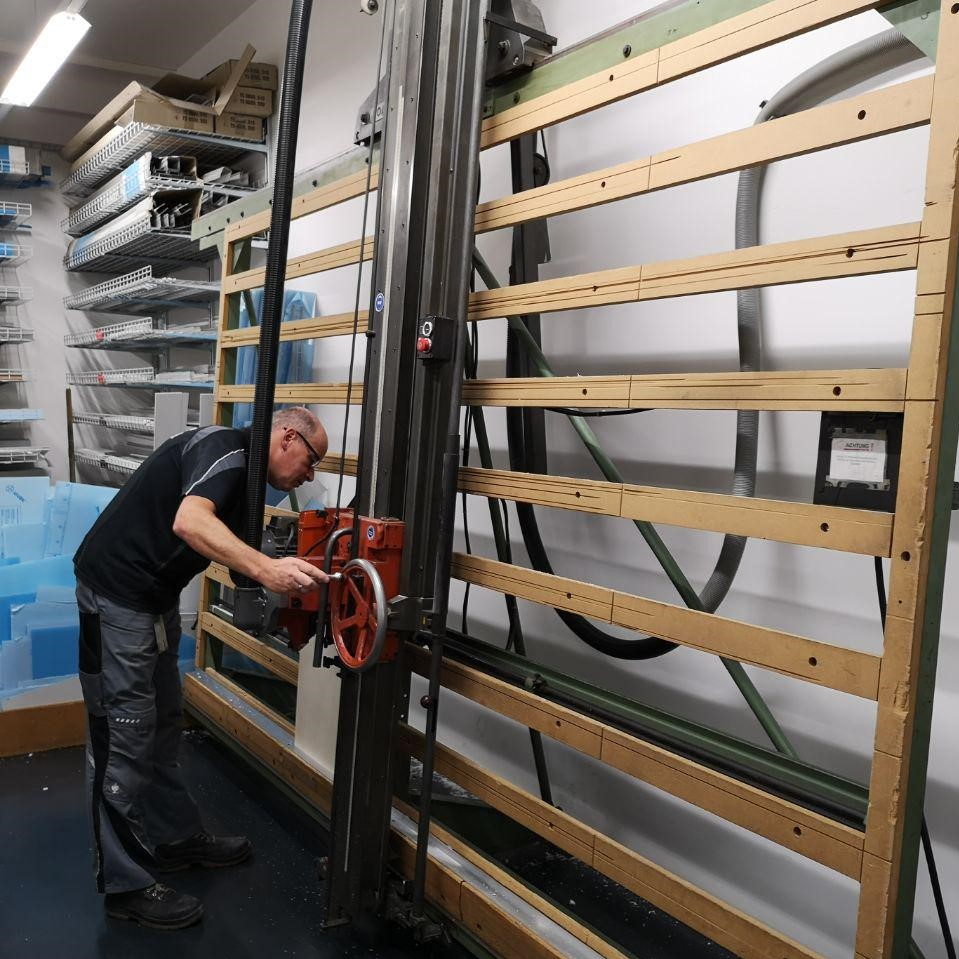
\includegraphics[width = 0.4\textwidth]{brice.jpg}
  \space{   }
  
\includegraphics[width = 0.4\textwidth]{bohren.jpg}
  \\}
 \vspace{1cm}
 
After one day of handicraft work, our box was finished and we ended the day by spraying the outer wall bright red. This can be seen in the picture on the left below.
 Next we had to glue the strips on a wooden board, which you can see in the picture on the right.
 
 \vspace{1cm}

{ \centering
  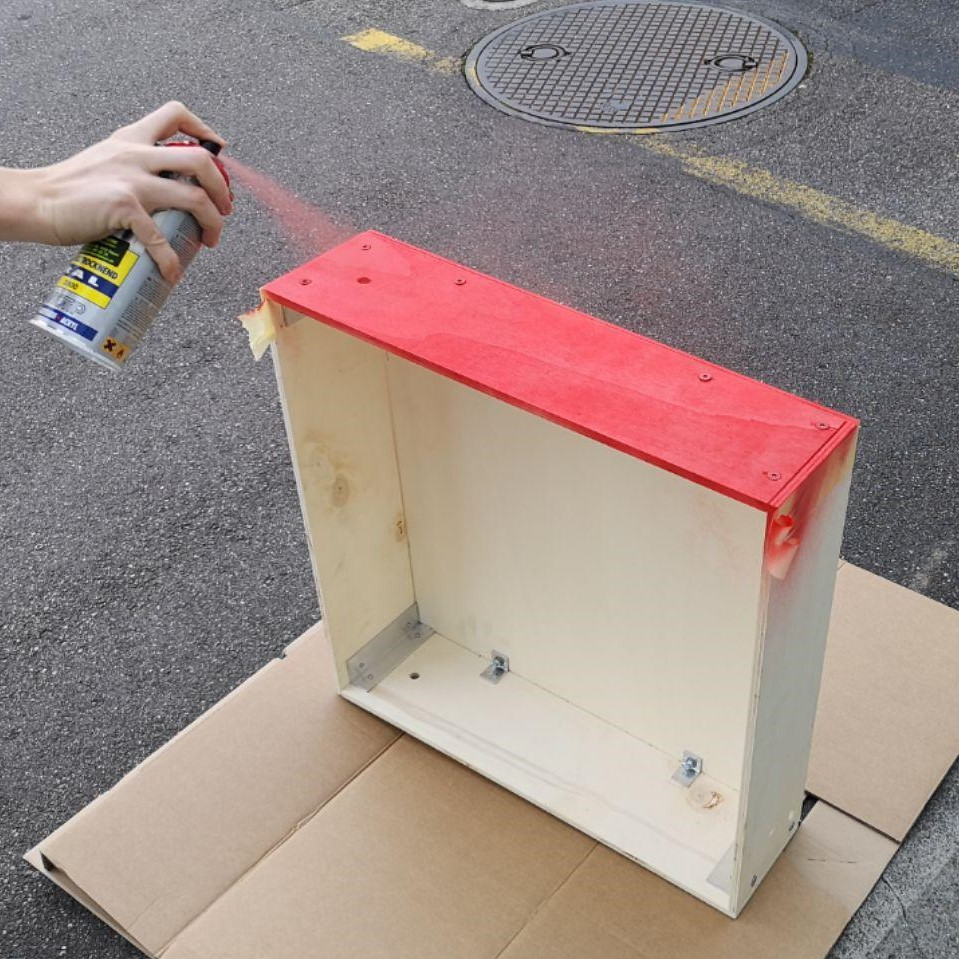
\includegraphics[width = 0.4\textwidth]{sprayen.jpg}
  \space{   }
  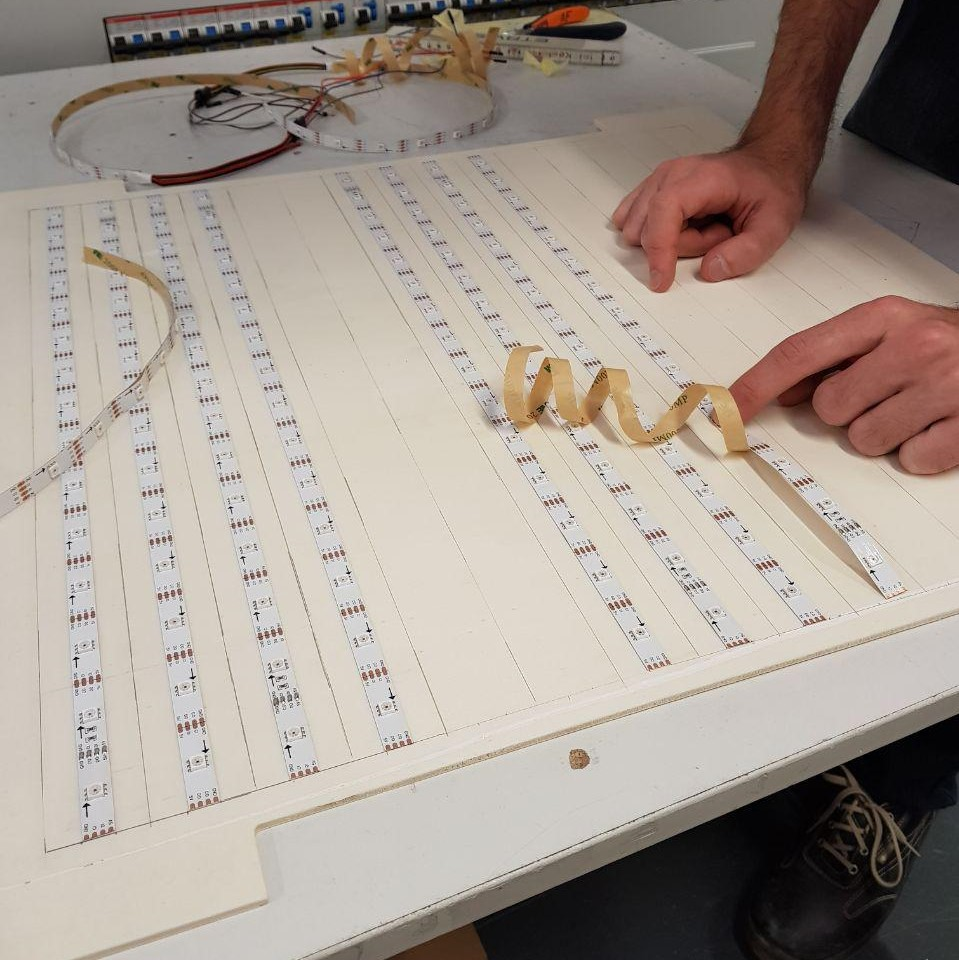
\includegraphics[width = 0.4\textwidth]{kleben.jpg}
  \\}
 \vspace{1cm}
 
Furthermore, we had to solder the strips together.
 Since none of us had any experience with soldering, we were surprised how nice it looked and that all of the LED strips were working correctly after the first try.
 Below you see a picture of one of us soldering (left) and the finished LED board (right).
 In the beginning we thought about adding paper walls between each LED, to get exact light squares per diode.
 As soon as we tried it, we both had the feeling that it looked nicer without these walls, hence we left them out.
 As for the distance between the acrylic glass (reference 4) and the light board, we decided to place them directly on top of each other.
 
 \vspace{1cm}

{ \centering
  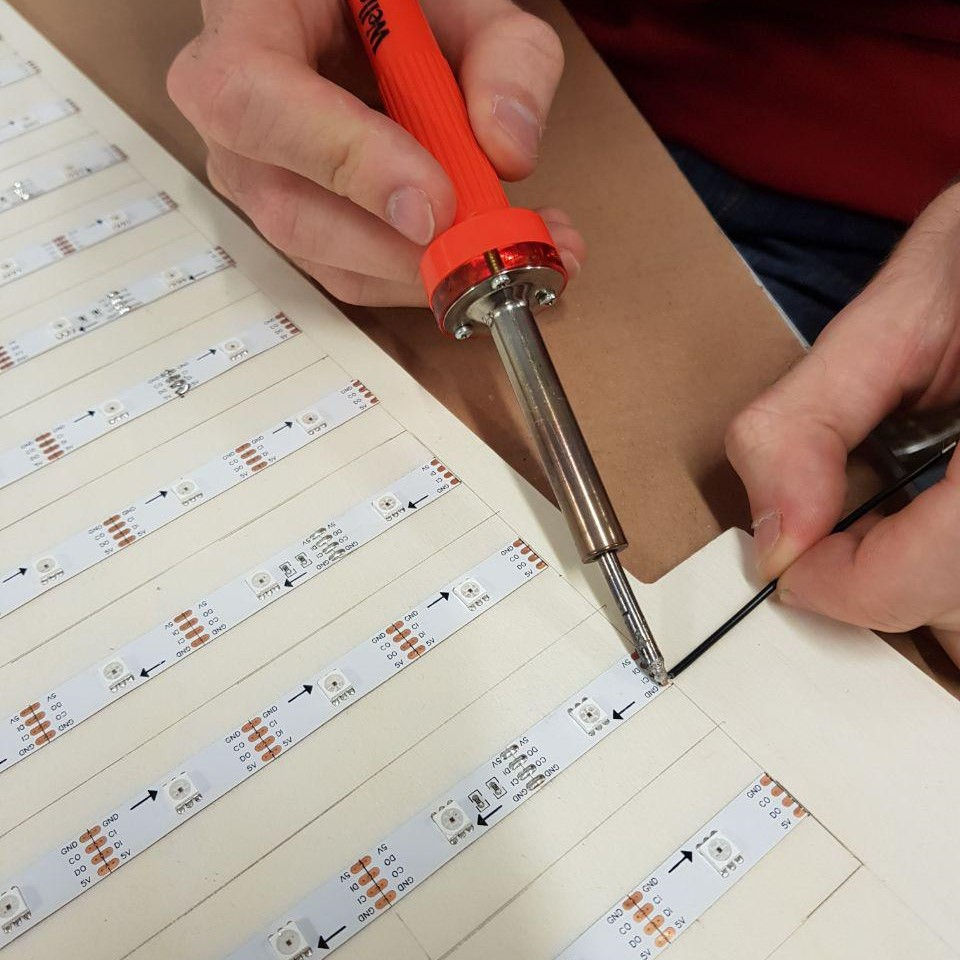
\includegraphics[width = 0.4\textwidth]{loten.jpg}
  \space{   }
  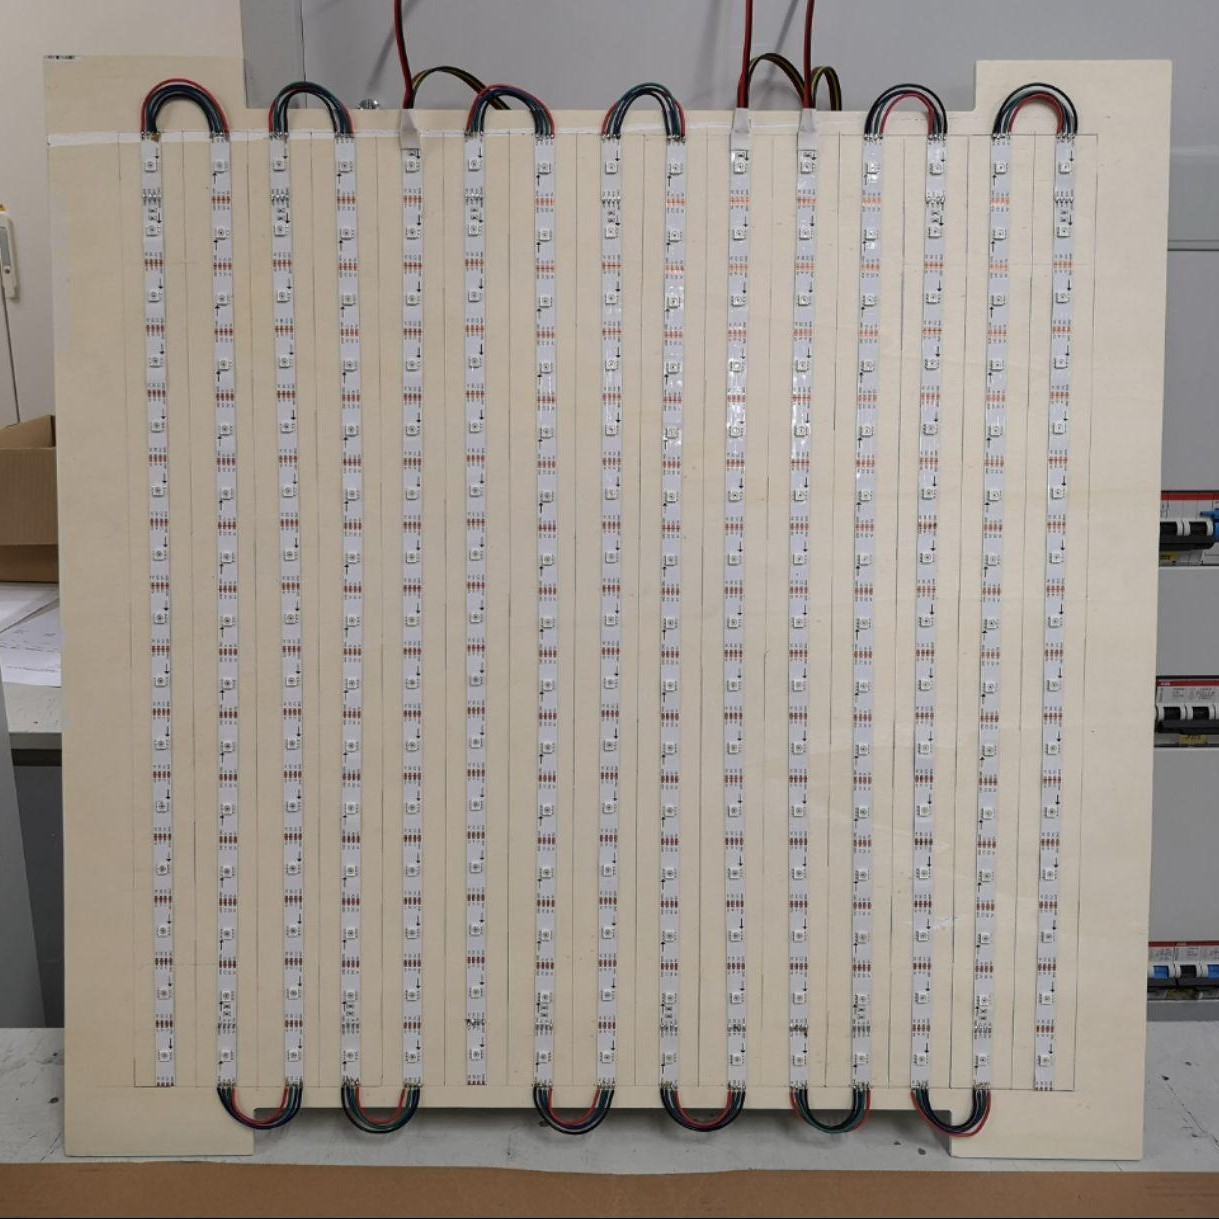
\includegraphics[width = 0.4\textwidth]{matrix.jpg}
  \\}
 \vspace{1cm}
 
\section{Coding}
Before we built the box, both of us started to try different things on the LEDs using the language C.
 We had to know exactly how they work and what order of information they expect, so they would display the desired colors at the right places.
 This could have been very difficult and time consuming, but luckily we came to the correct conclusions really fast.
 We also had to conclude that the LEDs are consuming too much energy for activating them all together.
 For this reason we chose to have three blocks of five strips each, in order to have only twelve bulbs blinking at once.
 
 Another reason for splitting it up was that 7.5 meters were too long to transport the data fast enough.
 In each of the blocks only four LEDs are shining at once, beginning with the first four, then the next four and so on.
 Because this happens very quickly, it looks like all of the 225 LEDs would be shining at once.
 The first result we had was very disappointing, as the LEDs flickered very much and the colors were inconsistent.
 By spending some time working on it, we made our code more efficient and reliable, which led to the satisfying result we got at the end.
 One big change was the replacement of the wiringPi library with direct gpio memory mapping, therefore the data could be passed to the strips with less overhead.

After the hardware part was finished and the LEDs could be managed, we started programming a demo and each of us a game.
 Since we had no working buttons yet, both of the games had a demo mode which was showed on the board.

We thought that with this done and only the buttons left, the biggest part of the project would have been done.
 But in fact, it was not.
 Our buttons are very imprecise, in fact one click triggers multiple interrupts.
 This is an unusable behavior, as for example while playing Raindrops, one might want to go one step to the left only but dies because one push leads to three steps.
 To avoid this, we introduced a timer minimizing the amount of clicks we are responding to during a certain interval.

\section{Conclusion}
First of all, we are happy that our project idea worked out and that our goals have been achieved within the given time frame.
 The games are fun to play, nice designed and with almost no flickering anymore the box provides a good gaming experience.
 The following pictures show the finished box, and our three games, TicTacToe, Raindrops and Snake (from top left to bottom right).
 
 \vspace{1cm}
 { \centering
  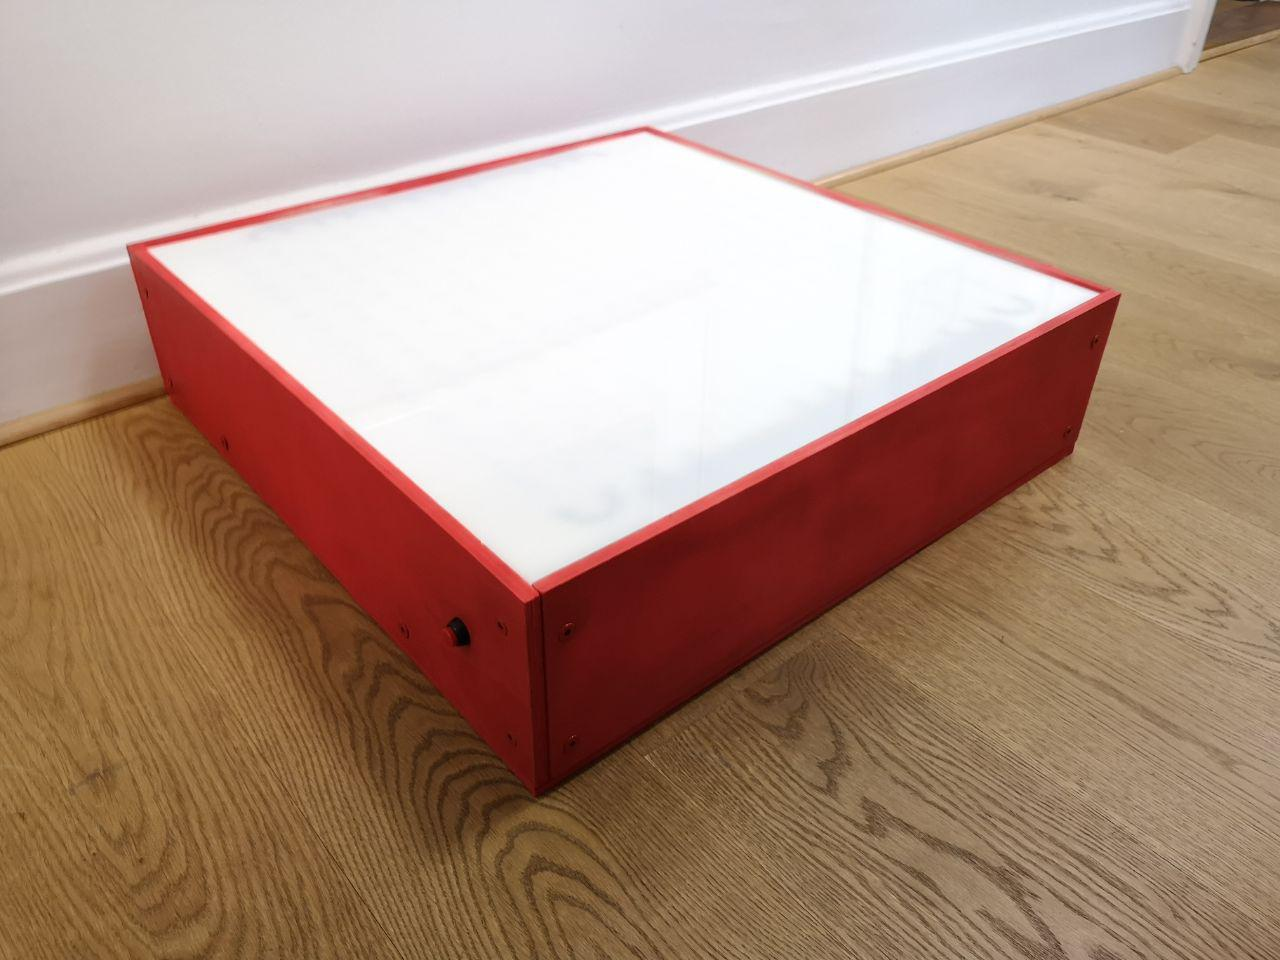
\includegraphics[width = 0.4\textwidth]{box.jpg}
  \space{   }
  
\includegraphics[width = 0.4\textwidth]{ttt.jpg}
  \\}
 \vspace{0.5cm}
 { \centering
 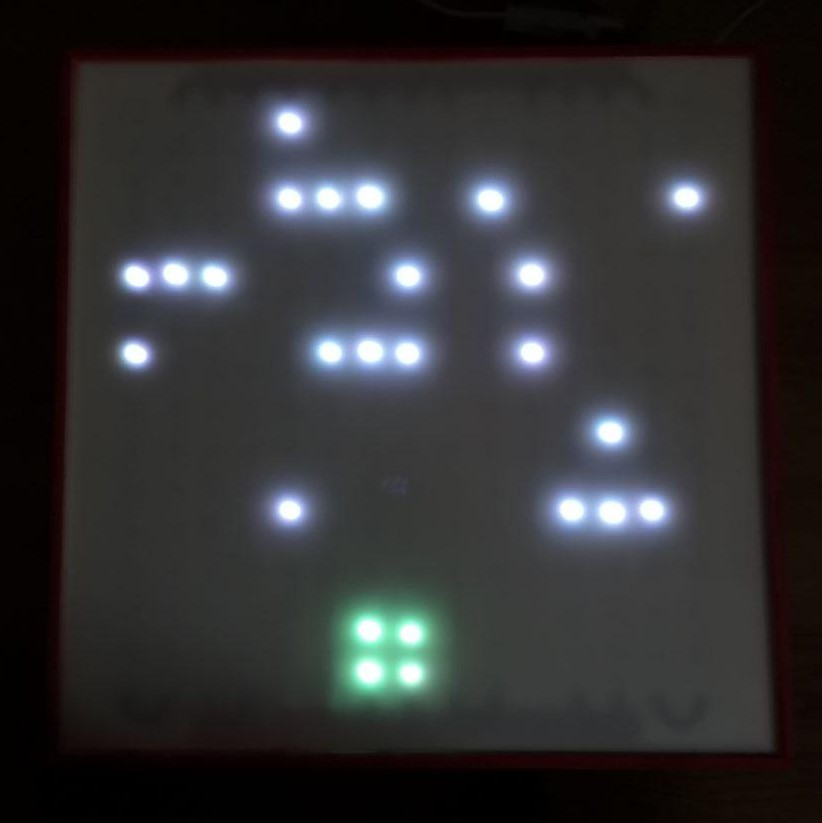
\includegraphics[width = 0.4\textwidth]{rd.jpg}
  \space{   }
  \includegraphics[width = 0.4\textwidth]{snake.jpg}
  \\}
  \vspace{1cm}

We developed in the Code-and-Fix model, for which reason we had a lot of refactoring and did things that didn't work with the first approach.
 If we would have made more brainstorming in the beginning, probably we would have found a more generic solution.
 
 In addition, because both of us were writing one game and we did not talk about a common structure before, they were not similar.
 When we put them together, we had to refactor a lot of things to have inherent code.

Furthermore, we should have taken notes about decisions and important bugs we removed during the process, since we forgot about some of them.
 When starting with the report, we had to think a lot about what we did and why, so we couldn't write this down directly, which took us a lot of time.

\section{References}

1) \href{https://cpldcpu.wordpress.com/2014/11/30/understanding-the-apa102-superled/}{\nolinkurl{APA102-description}}

2) \href{https://cpldcpu.wordpress.com/2014/01/14/light_ws2812-library-v2-0-part-i-understanding-the-ws2812/}{\nolinkurl{WS2812-description}}

3) \href{https://www.robotshop.com/de/de/squid-schalter-fur-raspberry-pi-von-monk-makes.html}{\nolinkurl{Squid-buttons}}

4) \href{https://www.plexiglas-shop.com/Products/PLWH72-GT-3-00-3050X2030-B-01-L.html}{\nolinkurl{Acrylic-glass}}

5) \href{https://www.eagb.ch}{\nolinkurl{EAGB}}

\end{document}